% ====================================================================
% JMP_seminar_beamer_v17.tex -- seminar deck, style revision of V16.
%
% Style model: the companion theory talk "Jobs and Well-Being Measurement".
% Short conceptual frame titles; slide bodies carry formal objects only
% (equations, figures, short labelled columns, citations); \vfill does the
% spacing; the narration lives in \note{}.  V16 and r6 are kept intact.
%
% Content: the V15 research-story report and results gallery.  Every numeral
% is a macro from deck_numbers_v17.tex (`make_deck_numbers_r6.py --v17`, read
% from reports/numbers_of_record_v15.json).  Figures are the V15 image files,
% unchanged.  Checks: `verify_deck_r6.py --deck v17`.  Build: build_deck_v17.py.
%
% Main deck: 16 frames.  Backup (after \appendix, after the conclusion): the
% two decomposition tables, the matched-household figure, equivalisation.
% EA is presented first as the prospect perspective and ATT as the
% attained-outcome benchmark; neither is designated primary.
% ====================================================================
\documentclass[10pt,aspectratio=169]{beamer}
% ====================================================================
% jmp_beamer_preamble.tex --- shared preamble for the JMP seminar deck.
%
% REUSED VERBATIM from the companion theory talk
%   beamer/reference/Theory_talk/slides/Presentation.tex
%     "Jobs and Well-Being Measurement" (Haydar and Maniquet)
% so that the two decks read as one visual family.  The elements carried
% over unchanged are marked [THEORY-TALK] below; everything else is an
% addition this deck needs and the theory talk does not.
%
% Consistency is the point: same class options, same theme, same accent
% colour, same frame numbering, same appendix handling, same visible-link
% convention, same note-page template, same two-agent sketch palette.
% ====================================================================

% ---- [THEORY-TALK] class, theme and the deep-red accent -------------
\usetheme{metropolis}
\definecolor{deepred}{RGB}{150,25,35}
\setbeamercolor{frametitle}{bg=deepred}
\setbeamertemplate{navigation symbols}{}
% metropolis-defined accents (safe: these beamercolors exist in metropolis)
\setbeamercolor{progress bar}{fg=deepred}
\setbeamercolor{title separator}{fg=deepred}
% frame number as current/total, in deep red
\metroset{numbering=fraction}
\setbeamercolor{footline}{fg=deepred}
% backup appendix: keep the main frame total at the running-order count
\usepackage{appendixnumberbeamer}
% VISIBLE link colours for rehearsal (internal hyperlinks in deep red)
\hypersetup{colorlinks=true,linkcolor=deepred,citecolor=deepred,urlcolor=deepred}

% ---- [THEORY-TALK] encoding, language, maths, tables, tikz ----------
\usepackage[utf8]{inputenc}
\usepackage[english]{babel}
\usepackage{amsmath}
\usepackage{amssymb}
\usepackage{amsfonts}
\usepackage{booktabs}
\usepackage[official]{eurosym}   % \euro --- this deck quotes euro magnitudes
\usepackage{tikz}
\usetikzlibrary{decorations.pathreplacing,arrows.meta,positioning,fit,backgrounds}

% ---- [THEORY-TALK] the two-agent sketch palette --------------------
% red = agent i / household A ; blue = agent h / household B
\definecolor{agenti}{RGB}{200,30,40}
\definecolor{agenth}{RGB}{20,80,200}

% ---- [THEORY-TALK] notes on a second screen (rehearsal view) -------
% The rehearsal build turns this on; the projection build leaves it off.
\usepackage{pgfpages}
% Long notes overflow the note column by default; render them smaller,
% ragged-right, with tight paragraph spacing so the full text stays
% legible and inside the frame on the second screen.
%
% This deck's notes are longer than the theory talk's -- several run past
% one note page at \scriptsize and produced overfull \vbox warnings.  The
% template below keeps the theory talk's look and adds two things it
% needs: \tiny with a tighter baseline, and an \allowbreak-friendly
% vertical box so a long note breaks across note pages instead of
% overflowing.  Hyphenation is relaxed so no line runs into the margin.
\setbeamertemplate{note page}{%
  \vspace{0.3em}\par
  {\tiny\setlength{\parskip}{0.45em}\setlength{\parindent}{0pt}%
   \setlength{\emergencystretch}{3em}%
   \linespread{1.05}\selectfont
   \raggedright\insertnote\par}%
}
% Notes are prose, not code: let TeX hyphenate freely rather than push a
% long word past the measure.
\hyphenpenalty=50
\tolerance=2000

\DeclareMathOperator*{\argmax}{arg\,max}

% ====================================================================
% ADDITIONS for this deck (not in the theory talk)
% ====================================================================

% ---- channel colours ------------------------------------------------
% One colour per decomposition channel, used consistently on every slide
% that names a channel.  Preferences take the theory talk's agent-red so
% the two decks agree on which side of the argument is which.
\definecolor{chpref}{RGB}{200,30,40}     % preferences   (= agenti)
\definecolor{chacc}{RGB}{20,80,200}      % job access    (= agenth)
\definecolor{chearn}{RGB}{200,120,20}    % earning opportunities
\definecolor{chneeds}{RGB}{40,120,70}    % endowments and needs
\definecolor{chenv}{RGB}{60,60,70}       % the whole environment

% ---- the paper's notation ------------------------------------------
% Audience-facing channel names are WORDS on the slides; these commands
% exist so the words are spelled the same way every time they appear.
\newcommand{\pref}{\textcolor{chpref}{preferences}}
\newcommand{\Pref}{\textcolor{chpref}{Preferences}}
\newcommand{\acc}{\textcolor{chacc}{job access}}
\newcommand{\Acc}{\textcolor{chacc}{Job access}}
\newcommand{\earn}{\textcolor{chearn}{earning opportunities}}
\newcommand{\Earn}{\textcolor{chearn}{Earning opportunities}}
\newcommand{\needs}{\textcolor{chneeds}{household endowments and needs}}
\newcommand{\Needs}{\textcolor{chneeds}{Household endowments and needs}}
\newcommand{\env}{\textcolor{chenv}{the environment}}
\newcommand{\Env}{\textcolor{chenv}{The environment}}

% Symbols.  The theory-paper symbols W, z, R, A, y appear ONLY where the
% companion paper is cited; the estimation notation is separate.
\newcommand{\Wmeasure}{W}                      % theory-paper measure
\newcommand{\Jset}{\mathcal{J}}                % theory-paper job space
\newcommand{\Wone}{W^{1}}                      % theory-paper W^1
\newcommand{\yref}{\mathbf{y}^{w}}             % theory-paper reference pay
\newcommand{\gopp}{g}                          % estimated offer density
\newcommand{\uutil}{u}                         % preference index
\newcommand{\Wmm}{\mathrm{W}}                  % money-metric welfare level

% ---- headline / caveat call-outs -----------------------------------
\newcommand{\headline}[1]{{\large\textcolor{deepred}{#1}}}
\newcommand{\caveat}[1]{{\footnotesize\textcolor{deepred}{#1}}}
% a number with its numerical-integration band
\newcommand{\wband}[2]{#1\,\ensuremath{\pm}\,#2}

% ---- the 25-minute variant ------------------------------------------
% Every frame carries \shortdeck (in the 25-minute running order) or
% \longdeck (45-minute only).  \DeckShort, set by the driver file, drops
% the \longdeck frames; the default keeps everything.
%
% The frozen plan's 25-minute running order is 16 slides, reached from the
% 23 by FIVE cuts and TWO merges:
%   CUT   -> backup : 9, 12, 17, 18, 22          (\longdeck)
%   MERGE           : 6+7 -> one slide, 10+11 -> one slide
% So three tags, not two.  A merged pair is written as two full frames for
% the 45-minute deck; in the short deck the SECOND of the pair drops and
% the first shows its merged content.  23 - 5 - 2 = 16.
%
% Usage:  \shortdeck{\begin{frame}...\end{frame}}     kept in both
%         \longdeck{\begin{frame}...\end{frame}}      45-minute only (cut)
%         \mergedaway{\begin{frame}...\end{frame}}    45-minute only (merged)
%         \ifDeckShort ... \else ... \fi              inline merged content
\newif\ifDeckShort\DeckShortfalse
\newcommand{\shortdeck}[1]{#1}                       % always kept
\newcommand{\longdeck}[1]{\ifDeckShort\else#1\fi}    % cut to backup at 25 min
\newcommand{\mergedaway}[1]{\ifDeckShort\else#1\fi}  % folded into the previous
% content shown only in the merged (25-minute) form of a slide
\newcommand{\mergedonly}[1]{\ifDeckShort#1\fi}

% ---- figure helper ---------------------------------------------------
% Every figure is a PDF from the frozen sprint set, included by name from
% beamer/figures/.  \deckfig{name}{width fraction} keeps the call sites
% uniform and makes a missing file fail loudly at compile time.
\graphicspath{{figures/}}
% Heights leave room for the frametitle, the one caption line every figure
% slide carries, and the metropolis footline -- a taller box overflows the
% frame and shows up as an overfull \vbox.
\newcommand{\deckfig}[2]{%
  \begin{center}\includegraphics[width=#2\textwidth,height=0.70\textheight,%
    keepaspectratio]{#1}\end{center}}
\newcommand{\deckfigtwo}[4]{%
  \begin{columns}[c,onlytextwidth]
  \column{0.49\textwidth}\includegraphics[width=\textwidth,height=0.60\textheight,%
    keepaspectratio]{#1}\\{\centering\scriptsize #2\par}
  \column{0.49\textwidth}\includegraphics[width=\textwidth,height=0.60\textheight,%
    keepaspectratio]{#3}\\{\centering\scriptsize #4\par}
  \end{columns}}

% ---- tables ---------------------------------------------------------
% Several slides carry a comparison table that is naturally wider than the
% text block.  \decktable shrinks one to the measure rather than letting it
% run into the margin (an overfull \hbox), and never enlarges a narrow one.
\newcommand{\decktable}[1]{%
  \begin{center}\resizebox{\textwidth}{!}{#1}\end{center}}

\endinput

\usepackage{array}
% deck_numbers_v17.tex -- GENERATED by make_deck_numbers_r6.py --v17.
% Do not edit by hand.  Every numeral on a V17 slide comes from here, and
% every value here is one entry of reports/numbers_of_record_v15.json,
% formatted only (no arithmetic).

\newcommand{\VCollectionYear}{2016}
\newcommand{\VIncomeYear}{2015}
\newcommand{\VNSingles}{1,540}
\newcommand{\VNCouples}{2,223}
\newcommand{\VCEqGiniSingles}{0.2633}
\newcommand{\VAttEqGiniSingles}{0.2498}
\newcommand{\VCEqGiniCouples}{0.2268}
\newcommand{\VAttEqGiniCouples}{0.1974}
\newcommand{\VKFreeSingles}{41}
\newcommand{\VKFreeRumA}{10}
\newcommand{\VKFreeRumB}{16}
\newcommand{\VRumGap}{141.64}
\newcommand{\VMaeSingles}{0.0140}
\newcommand{\VMaeRumA}{0.0273}
\newcommand{\VMaeRumB}{0.0264}
\newcommand{\VMatchedAccessRatio}{14.5}
\newcommand{\VMatchedWageGap}{11.5}
\newcommand{\VMatchedEmpShareA}{0.75}
\newcommand{\VMatchedEmpShareB}{0.17}
\newcommand{\VEAOppMin}{7.9}
\newcommand{\VEAOppMax}{21.3}
\newcommand{\VEASingOppRaw}{14.8}
\newcommand{\VEASingOppEq}{20.3}
\newcommand{\VEACoupOppRaw}{21.3}
\newcommand{\VEACoupOppEq}{7.9}
\newcommand{\VEASingRatioRaw}{3.3}
\newcommand{\VEASingRatioEq}{3.2}
\newcommand{\VEASingPhiARaw}{0.01812}
\newcommand{\VEASingPhiBRaw}{0.00555}
\newcommand{\VEASingPhiAEq}{0.02183}
\newcommand{\VEASingPhiBEq}{0.00673}
\newcommand{\VEACoupPhiARaw}{0.00667}
\newcommand{\VEACoupPhiBRaw}{0.02049}
\newcommand{\VEACoupPhiAEq}{0.00449}
\newcommand{\VEACoupPhiBEq}{0.00504}
\newcommand{\VEACoupPrefRaw}{0.00291}
\newcommand{\VEACoupPrefEq}{$-$0.00212}
\newcommand{\VAttOppMin}{1.9}
\newcommand{\VAttOppMax}{6.7}
\newcommand{\VAttSingOppRaw}{2.4}
\newcommand{\VAttSingOppEq}{1.9}
\newcommand{\VAttCoupOppRaw}{6.7}
\newcommand{\VAttCoupOppEq}{3.5}
\newcommand{\VAttSingPhiARaw}{0.0016}
\newcommand{\VAttSingPhiBRaw}{0.0040}
\newcommand{\VAttSingPhiAEq}{0.0013}
\newcommand{\VAttSingPhiBEq}{0.0034}
\newcommand{\VAttCoupPhiARaw}{0.0009}
\newcommand{\VAttCoupPhiBRaw}{0.0128}
\newcommand{\VAttCoupPhiAEq}{0.0007}
\newcommand{\VAttCoupPhiBEq}{0.0062}
\newcommand{\VPolicyYear}{2015}
\newcommand{\VNDraws}{100}
\newcommand{\VNOcc}{4}
\newcommand{\VHoursFloor}{5}
\newcommand{\VHoursCap}{70}
\newcommand{\VWageLo}{2}
\newcommand{\VWageHi}{590}

\graphicspath{{../manuscript/figures/v13/}{../manuscript/figures/v11/}{../manuscript/figures/v5/}}
\metroset{sectionpage=none}
\ifdefined\RehearsalDeck
  \setbeameroption{show notes on second screen=right}
\fi
% the theory talk's note page
\setbeamertemplate{note page}{%
  \vspace{0.3em}\par
  {\scriptsize\setlength{\parskip}{0.5em}\setlength{\parindent}{0pt}%
   \raggedright\insertnote\par}%
}
% the theory talk's plain frame title (the preamble's two-line headline box is not used)
\setbeamertemplate{frametitle}[default]
\setbeamerfont{frametitle}{size=\large}
\setbeamerfont{title}{size=\Large}

\title{Unequal Job Opportunities and Well-Being Inequality}
\subtitle{A Latent-Jobs Structural Decomposition}
\author{Hisham Haydar}
\institute{University of Luxembourg and LISER}
\date{}

\begin{document}

% ==================================================================== 1
\begin{frame}[plain,noframenumbering]
\vfill
{\Large\bfseries\inserttitle\par}
\vspace{0.4em}
{\large\insertsubtitle\par}
\vspace{0.9em}
{\color{deepred}\rule{0.80\textwidth}{1pt}}\par
\vspace{0.9em}
{\normalsize\insertauthor\par}
{\small\insertinstitute\par}
\vfill
\note{Thank you. This talk asks how much of the inequality in money-metric
well-being goes with unequal job opportunities rather than with differences in
what people prefer. I build the answer in four steps: a model of labour supply
as choice among latent jobs, which separates preferences from opportunities;
two ways of turning choices into euros of well-being; counterfactuals that
equalise one source of heterogeneity at a time; and a Shapley rule that
allocates the change. The punchline is that the answer depends on the welfare
question: prospects or attained outcomes.}
\end{frame}

% ==================================================================== 2
\begin{frame}
\frametitle{Motivation}
\vfill
\begin{columns}[T,onlytextwidth]
\column{0.46\textwidth}
\centering
\textbf{Observed}\\[0.5em]
{\Large $C_i$}\\[0.5em]
{\small Gini of consumption}\\[0.3em]
{\small single adults \VCEqGiniSingles{} \quad couples \VCEqGiniCouples{}}

\column{0.46\textwidth}
\centering
\textbf{Well-being}\\[0.5em]
{\Large $M_i$}\\[0.5em]
{\small Gini of the attained-bundle money metric}\\[0.3em]
{\small single adults \VAttEqGiniSingles{} \quad couples \VAttEqGiniCouples{}}
\end{columns}
\vfill
\begin{center}
low earnings \quad$\Longleftarrow$\quad tastes \quad \textbf{or} \quad opportunities \quad \textbf{or} \quad resources
\end{center}
\vfill
{\footnotesize equivalised, household-weighted, within each population}
\note{Two people can work the same hours for the same hourly pay and be very
differently placed. One chose that job from several that were open; the other
took the only offer available. Their incomes are identical and their
circumstances are not.

Low earnings can describe someone who values leisure and chose short hours,
someone who cannot obtain a well-paid job, or someone whose household resources
make a different arrangement affordable. An income distribution records
outcomes with these explanations already mixed in.

The numbers make the point in the French data: once the leisure a job costs is
valued, the dispersion of well-being is not the dispersion of consumption. These
are within-population dispersion comparisons, not welfare-loss estimates, and
single-adult and couple households are separate populations that I never
compare with each other.}
\end{frame}

% ==================================================================== 3
\begin{frame}
\frametitle{The conflict}
\vfill
\begin{columns}[T,onlytextwidth]
\column{0.46\textwidth}
\centering
\textbf{Compensation}\\[0.35em]
{\small unequal job opportunities should not become unequal well-being}
\column{0.46\textwidth}
\centering
\textbf{Responsibility}\\[0.35em]
{\small preference-based choices should not be compensated}
\end{columns}
\vfill
\begin{center}
{\large Compensation \qquad vs.\qquad Responsibility}\\[0.8em]
$\nexists\, W:\quad \text{Full Compensation}\ \wedge\ \text{Full Responsibility}$
\end{center}
\begin{flushright}\small[Fleurbaey \& Maniquet]\end{flushright}
\vfill
\note{Before any data, the conflict that makes this paper necessary.

A fair well-being comparison would like to respect two principles. The first is
compensation: people should not end up worse off because they face worse job
opportunities. The second is responsibility: people should be held responsible
for their preferences, their tastes for work, leisure and consumption, so a
choice that reflects taste should not generate a compensation claim.

Each principle is attractive on its own, but they cannot both be imposed in
full: no well-being measure satisfies full compensation and full
responsibility together. The literature, following Fleurbaey and Maniquet, is
organised around compromises.

The empirical consequence is the reason for this paper. To know what to
compensate, we must separate what people prefer from what they can reach. And
observed choices mix the two.}
\end{frame}

% ==================================================================== 4
\begin{frame}
\frametitle{Research question}
\vfill
\begin{block}{}
How much inequality in money-metric well-being is associated with unequal job
opportunities rather than heterogeneous preferences, once labour supply is
modelled as choice among latent jobs?
\end{block}
\vfill
\begin{enumerate}\itemsep0.6em
  \item Do observed labour-supply choices reflect preferences alone, or also
        heterogeneous latent job opportunities?
  \item How do conclusions differ when welfare evaluates the attained bundle
        versus the ex-ante opportunity prospect?
  \item In a restricted P/A/B decomposition, how much welfare inequality is
        associated with preferences, local access, and earning opportunities?
\end{enumerate}
\vfill
\note{The whole talk on one slide. The first subquestion is behavioural: can
we read preferences off choices, or do opportunities get in the way? The second
is normative: once well-being is valued in euros, does it matter whether we
value the prospect a household faces or the outcome it attains? The third is
the accounting: in a restricted decomposition with preferences, local access and
earning opportunities as the three channels, how is inequality allocated?

Note the word associated. Nothing in this talk is a causal claim.}
\end{frame}

% ==================================================================== 5
\begin{frame}
\frametitle{Literature and gap}
\vfill
\begin{columns}[T,onlytextwidth]
\column{0.31\textwidth}
\centering
\textbf{Latent jobs}\\[0.35em]
{\footnotesize Aaberge, Dagsvik \& Str{\o}m\\ Dagsvik \& Jia\\ Cap\'eau, Decoster \& Dekkers}
\column{0.31\textwidth}
\centering
\textbf{Money metrics}\\[0.35em]
{\footnotesize Fleurbaey \& Maniquet\\ Decoster \& Haan\\ Jacquet, Jia \& Thoresen}
\column{0.31\textwidth}
\centering
\textbf{Decomposition}\\[0.35em]
{\footnotesize Shorrocks\\ Creedy \& H\'erault\\ M\"uhlhan}
\end{columns}
\vfill
\begin{center}
{\small reforms and \emph{changes}} \quad$\longrightarrow$\quad {\small a \emph{level} of well-being inequality}\\[0.5em]
preferences \ vs.\ opportunities, inside an estimated latent-jobs model
\end{center}
\vfill
\note{Every ingredient has antecedents; the contribution is the combination and
the empirical answer.

Labour supply as choice among latent jobs, with preference and opportunity
components jointly estimated under maintained restrictions, is due to Aaberge,
Dagsvik and Str{\o}m, developed by Dagsvik and Str{\o}m and by Dagsvik and Jia,
and set out for applied work by Cap\'eau, Decoster and Dekkers, who already cover
singles and couples.

Money-metric evaluation with such models exists, but it evaluates a change
between policy regimes. The normative literature following Fleurbaey and
Maniquet, with Decoster and Haan and Bargain and co-authors, shows how the
reference encodes compensation and responsibility.

The closest decompositions, Creedy and H\'erault and M\"uhlhan, decompose a
change between situations. Our object is a cross-sectional level of well-being
inequality, decomposed into preferences and opportunities inside an estimated
latent-jobs model. The Shapley rule itself is inherited from Shorrocks; no new
allocation principle is claimed.}
\end{frame}

% ==================================================================== 6
\begin{frame}
\frametitle{Job packages}
\vfill
\begin{center}
$j=(e,\,k,\,h,\,w)$ \qquad \VNOcc{} occupation groups \qquad $C_i(j)$ priced through EUROMOD
\end{center}
\slideeq{$\displaystyle v_i(j)=L_i(j)+\beta_c\log\!\left(\frac{C_i(j)}{\lambda_c}\right)$}
\begin{columns}[T,onlytextwidth]
\column{0.31\textwidth}\centering
$L_i$\\ {\footnotesize value of leisure: age; children for women}
\column{0.31\textwidth}\centering
$\beta_c$\\ {\footnotesize weight on log consumption, estimated}
\column{0.31\textwidth}\centering
$\lambda_c$\\ {\footnotesize units convention}
\end{columns}
\vfill
\note{In words: a household's systematic value of a job is the value of the
leisure it leaves plus the log of the consumption it pays.

A job is a package: an employment state, one of four occupation groups, weekly
hours and an hourly wage. Every package is run through the French tax-benefit
system, so consumption is the household's actual disposable income at that job.
A single adult chooses one package; a couple chooses a pair under a shared
budget, and the leisure term sums both spouses' terms.

The split between leisure and consumption matters later: consumption is
observable in euros and leisure is not, and the split is what turns a utility
gap into a proportional consumption adjustment in both welfare measures. The
household-specific leisure coefficients are the preference channel. The child
term is a reduced-form time-constraint shifter, not pure taste.}
\end{frame}

% ==================================================================== 7
\begin{frame}
\frametitle{Opportunities: the choice probability}
\slideeq{$\displaystyle P_i(j)=\frac{\exp\{v_i(j)\}\,g_i(j)}{\displaystyle\int\exp\{v_i(k)\}\,g_i(k)\,d\nu(k)}$}
\begin{columns}[T,onlytextwidth]
\column{0.23\textwidth}\centering
\textcolor{chacc}{\textbf{access}}\\ {\footnotesize employment mass}
\column{0.23\textwidth}\centering
\textbf{hours}\\ {\footnotesize bands}
\column{0.23\textwidth}\centering
\textbf{occupation}\\ {\footnotesize by sex}
\column{0.23\textwidth}\centering
\textcolor{chearn}{\textbf{wage offers}}\\ {\footnotesize education, experience}
\end{columns}
\vfill
\begin{center}
{\small valued \quad \textbf{or} \quad plentiful}
\end{center}
\vfill
\note{In words: the probability of being seen in a job is its value times its
availability, normalised over all jobs.

The function g is the household's opportunity density: how intensely a package
is available to it before any choice. A job is chosen often when it is valued
or when it is plentiful. If everyone faced the same density we would be back to
a standard model, in which every difference in behaviour must be a difference
in taste. Because the density is household-specific, part of behaviour can be
attributed to reachability.

The density has four blocks. Access, the employment mass, moves with local
unemployment exposure, region, urban or rural location, and year. Hours are a
step function over bands. Occupation availability is sex-specific. Wage offers
are log-normal, located by education and experience.

Separation rests on maintained restrictions, not tested ones: smooth
preferences against banded hours opportunities; local shifters excluded from
preferences; wage offers independent of hours given occupation. The regional
variation is not a causal design.}
\end{frame}

% ==================================================================== 8
\begin{frame}
\frametitle{Data and EUROMOD}
\vfill
\begin{columns}[T,onlytextwidth]
\column{0.46\textwidth}
\centering
\textbf{EU-SILC France}\\[0.5em]
{\small collected \VCollectionYear{}, incomes \VIncomeYear{}}\\[0.5em]
{\small \VNSingles{} single-adult households}\\
{\small \VNCouples{} couple households}

\column{0.46\textwidth}
\centering
\textbf{EUROMOD}\\[0.5em]
{\small French \VPolicyYear{} policy system}\\[0.5em]
$h\in[\VHoursFloor,\VHoursCap]$ \quad $w\in[\VWageLo,\VWageHi]$\\[0.3em]
{\small \VNDraws{} priced alternatives per household}
\end{columns}
\vfill
\note{The data are French EU-SILC, collected in the year on the slide, with
incomes referring to the previous year. Taxes, benefits and disposable income
come from EUROMOD under the policy system in force over the income period.

The samples are single-adult and couple households with every adult of working
age, not in education and not receiving a pension. Multi-generational
households and same-sex couples are outside the estimated population, so no
result extends to them. The two samples are estimated separately.

Hours are in hours per week and wages in euros per hour; those are the supports
the opportunity densities are defined on. Each household's likelihood is
evaluated on its observed job plus a set of sampled alternatives, each run
through the tax-benefit model. Sampling is a computational device, not an
offer: it enters no welfare measure.}
\end{frame}

% ==================================================================== 9
\begin{frame}
\frametitle{Estimation}
\vfill
\begin{columns}[T,onlytextwidth]
\column{0.46\textwidth}
\centering
\textbf{Household-specific opportunities}\\[0.5em]
{\small free coordinates \VKFreeSingles{}}\\
{\small population fit \VMaeSingles{}}

\column{0.46\textwidth}
\centering
\textbf{Common opportunities}\\[0.5em]
{\small free coordinates \VKFreeRumA{} \,/\, \VKFreeRumB{}}\\
{\small population fit \VMaeRumA{} \,/\, \VMaeRumB{}}
\end{columns}
\vfill
\begin{center}
criterion worse by at least \VRumGap{}\\[0.5em]
{\large choices reflect opportunities, not preferences alone}
\end{center}
\vfill
{\footnotesize single adults; population fit is the mean absolute deviation of predicted from observed moments}
\note{The first subquestion. Take away the household-specific opportunity
block, re-estimate everything else, and the model does worse: on the same
households, the same sampled alternatives and the same criterion.

The two benchmarks are a common opportunity distribution with re-estimated
preferences, and a common opportunity shape with employment and hours moved
into utility. The deterioration is concentrated where the opportunity block
does its work: population fit roughly doubles its error, and occupation margins
deteriorate by an order of magnitude.

I do not turn this into a likelihood-ratio test, because the sampled-alternative
criterion is not the likelihood of the observed data. A better criterion does
not by itself establish that a mechanism has been identified.

Fit is not perfect either. The observed concentration at exactly thirty-seven
hours is underpredicted in every group, and extensive-margin accuracy for men is
withheld because numerical integration error is too large relative to sampling
variation.}
\end{frame}

% ==================================================================== 10
\begin{frame}
\frametitle{Welfare}
\begin{center}
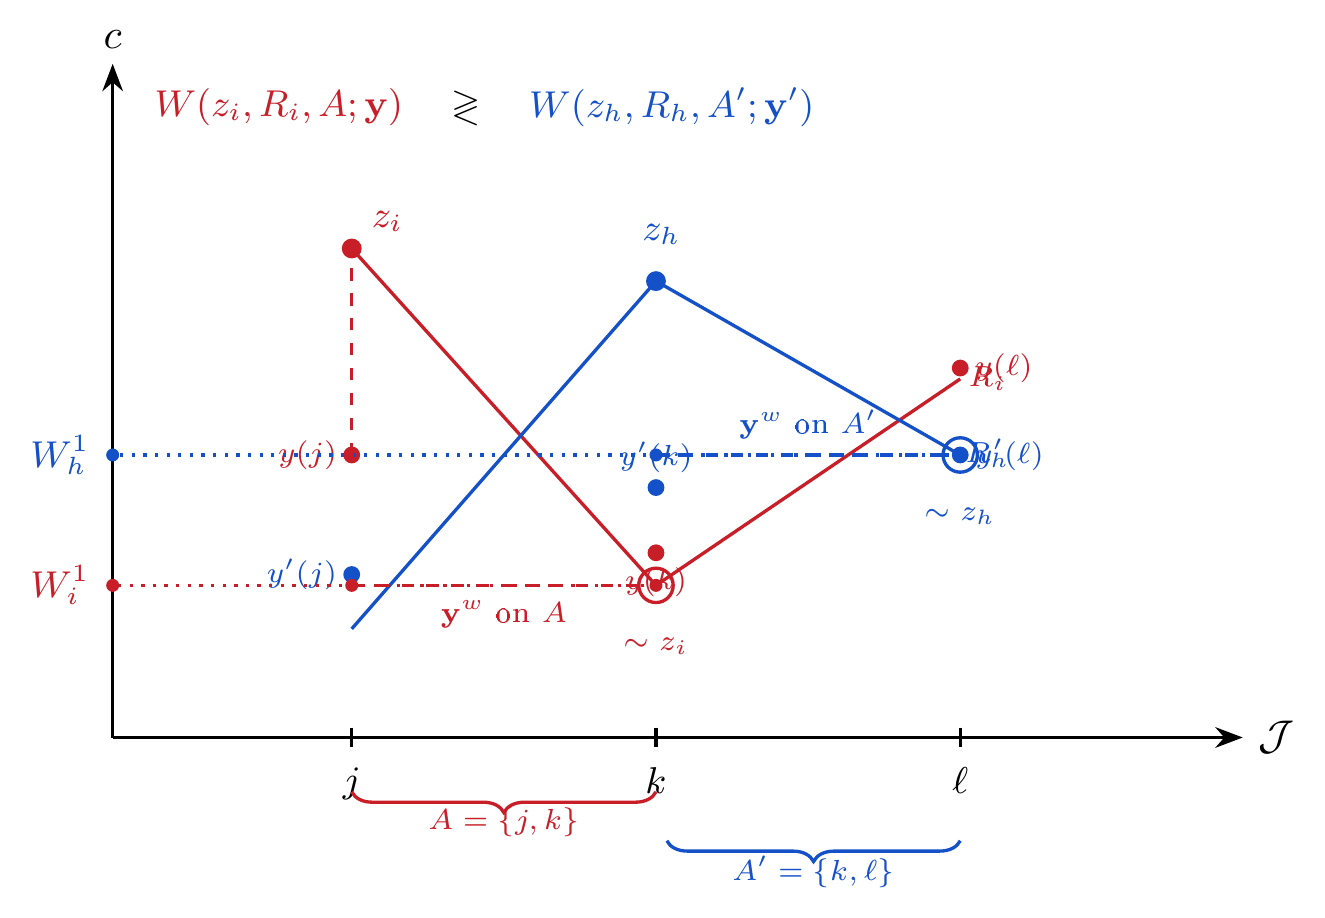
\includegraphics[height=0.64\textheight,width=\textwidth,keepaspectratio]{theory_w1.png}
\end{center}
{\footnotesize Own-set equal-consumption equivalents: each individual gets a common consumption on every job in their own ability set; the level at which the preferred job is indifferent to the attained bundle is their money metric, comparable across individuals. Adapted from Haydar and Maniquet (2026), work in progress.\par}
\note{Estimated utility is not an interpersonal welfare index: preferences
differ, so the same utility number means different things for different people.
To compare households, each situation is translated into euros through an
indifference condition with an explicit reference. The choice of reference is
the welfare question.

Both money metrics in this paper descend from this construction in the
companion theory paper. Each individual is evaluated with their own preferences
and their own set of jobs. Give every job in that set the same consumption; the
individual then prefers one of them, and the consumption at which that job is
exactly as good as the attained bundle is their money metric. The point is that
these metrics are comparable across people whose preferences and job sets
differ.

The figure is a theoretical illustration with no estimated value in it. The
next two slides take the construction to the data in two ways: applied to the
whole estimated prospect, and applied to the outcome attained.}
\end{frame}

% ==================================================================== 11
\begin{frame}
\frametitle{Ex-ante prospect welfare}
\slideeq{$\displaystyle\begin{gathered}
  J_i=\int e^{L_i(j)}\Big(\tfrac{C_i(j)}{\lambda_c}\Big)^{\beta_c}\,\widehat g_i(j)\,d\nu(j),
  \qquad
  H_i=\int e^{L_i(j)}\,\widehat g_i(j)\,d\nu(j),
  \\[0.35em]
  M^{\mathrm{EA}}_i=\lambda_c\exp\!\Big\{\tfrac{\log J_i-\log H_i}{\beta_c}\Big\}
  \end{gathered}$}
\begin{columns}[T,onlytextwidth]
\column{0.31\textwidth}\centering
$J_i$\\ {\footnotesize the actual prospect}
\column{0.31\textwidth}\centering
$H_i$\\ {\footnotesize same jobs, equal pay}
\column{0.31\textwidth}\centering
$M^{\mathrm{EA}}_i$\\ {\footnotesize flat-consumption equivalent}
\end{columns}
\vfill
\note{In words: EA is the constant monthly consumption at which a prospect with
the household's own jobs and availability, but equal pay everywhere, is worth
exactly as much as the prospect it actually faces.

J values the household's actual prospect over its whole estimated opportunity
environment: every job enters, weighted by how available it is and how much it
is valued. H is the reference: the same jobs, the same availability and the same
preferences, with pay differences removed. Opportunities enter welfare
directly: access moves which jobs carry weight; earning opportunities move what
they pay. A common rescaling of the opportunity density cancels.

I show this perspective first because this talk is about opportunities; that is
an order of presentation, not a ranking.

Under the extreme-value shocks, log J is the expected utility of the best
reachable job up to a constant, so the measure treats taste-shock variety as part
of what makes a rich prospect valuable. That is a normative position, not a
consequence of estimation, and I flag it. The ex-ante calculation passed its
numerical checks, which certifies the computation, not the model's assumptions.}
\end{frame}

% ==================================================================== 12
\begin{frame}
\frametitle{Attained-bundle welfare}
\slideeq{$\displaystyle M^{\mathrm{att}}_i=C^{\mathrm{obs}}_i\exp\!\left\{\frac{L_i(j^{\mathrm{obs}}_i)-L_i(o)}{\beta_c}\right\}$}
\begin{columns}[T,onlytextwidth]
\column{0.46\textwidth}\centering
$o$\\ {\footnotesize non-employment, reachable by all}
\column{0.46\textwidth}\centering
$j^{\mathrm{obs}}_i$\\ {\footnotesize the only route for opportunities}
\end{columns}
\vfill
\note{In words: ATT is observed consumption, adjusted by the leisure the job
costs relative to not working, converted at the rate one over the consumption
weight.

The reference is non-employment, which every household can reach. The general
construction evaluates the attained bundle against the job the household would
most prefer if all jobs paid the same; on the current empirical domain that job
is non-employment for every household, so the measure coincides with the
staying-home equivalent. That is a verified property of this specification, not
a general theorem.

Opportunities matter only through which job is attained and what it pays; once
that job is fixed, jobs not taken play no role. For non-workers the measure
equals observed consumption; for workers it lies below by the value of the
leisure given up.

The two measures answer different welfare questions: one values the prospect,
the other the attained outcome. Neither corrects the other.}
\end{frame}

% ==================================================================== 13
\begin{frame}
\frametitle{Inequality and Shapley decomposition}
\vfill
\begin{columns}[T,onlytextwidth]
\column{0.23\textwidth}\centering
\textcolor{chpref}{\textbf{P}}\\ {\footnotesize preferences: age, children}
\column{0.23\textwidth}\centering
\textcolor{chacc}{\textbf{A}}\\ {\footnotesize local unemployment exposure, region, urban or rural location, year}
\column{0.23\textwidth}\centering
\textcolor{chearn}{\textbf{B}}\\ {\footnotesize wage-offer location}
\column{0.23\textwidth}\centering
\textcolor{chneeds}{\textbf{held fixed}}\\ {\footnotesize household resources, needs and composition}
\end{columns}
\slideeq{$\displaystyle\phi^p_k=\sum_{S\subseteq\{P,A,B\}\setminus\{k\}}\frac{|S|!\,(3-|S|-1)!}{3!}\Big[v^p(S\cup\{k\})-v^p(S)\Big]$}
\begin{center}
$v^p(S)=I^p(\varnothing)-I^p(S)$ \qquad $I^p$: household-weighted Gini of $M^p$
\end{center}
\vfill
\note{In words: a channel's Shapley contribution is its marginal effect on
inequality, averaged over every order in which the three equalisations can be
introduced; the three contributions add up exactly to the total change.

P equalises the systematic preference shifters: age profiles and the
child-related shifter. A equalises local access: local unemployment exposure,
region, urban or rural location, and year. It is local access, not total
opportunity: personal occupation access and the hours density are left as
estimated. B equalises the systematic wage-offer location, not wage dispersion.
Household resources, needs and composition are held fixed in every coalition
and receive no share.

Each coalition is a full structural counterfactual: coefficients never change,
welfare is recomputed for every household under each perspective, and
inequality is measured again. The same operators and rule are applied to both
perspectives, which is what makes their orderings comparable. Contributions are
signed. Adding resources, needs and composition as a fourth channel is a
planned extension; access plus earnings would remain the opportunity component.}
\end{frame}

% ==================================================================== 14
\begin{frame}
\frametitle{Results: prospects versus attained outcomes}
\begin{center}
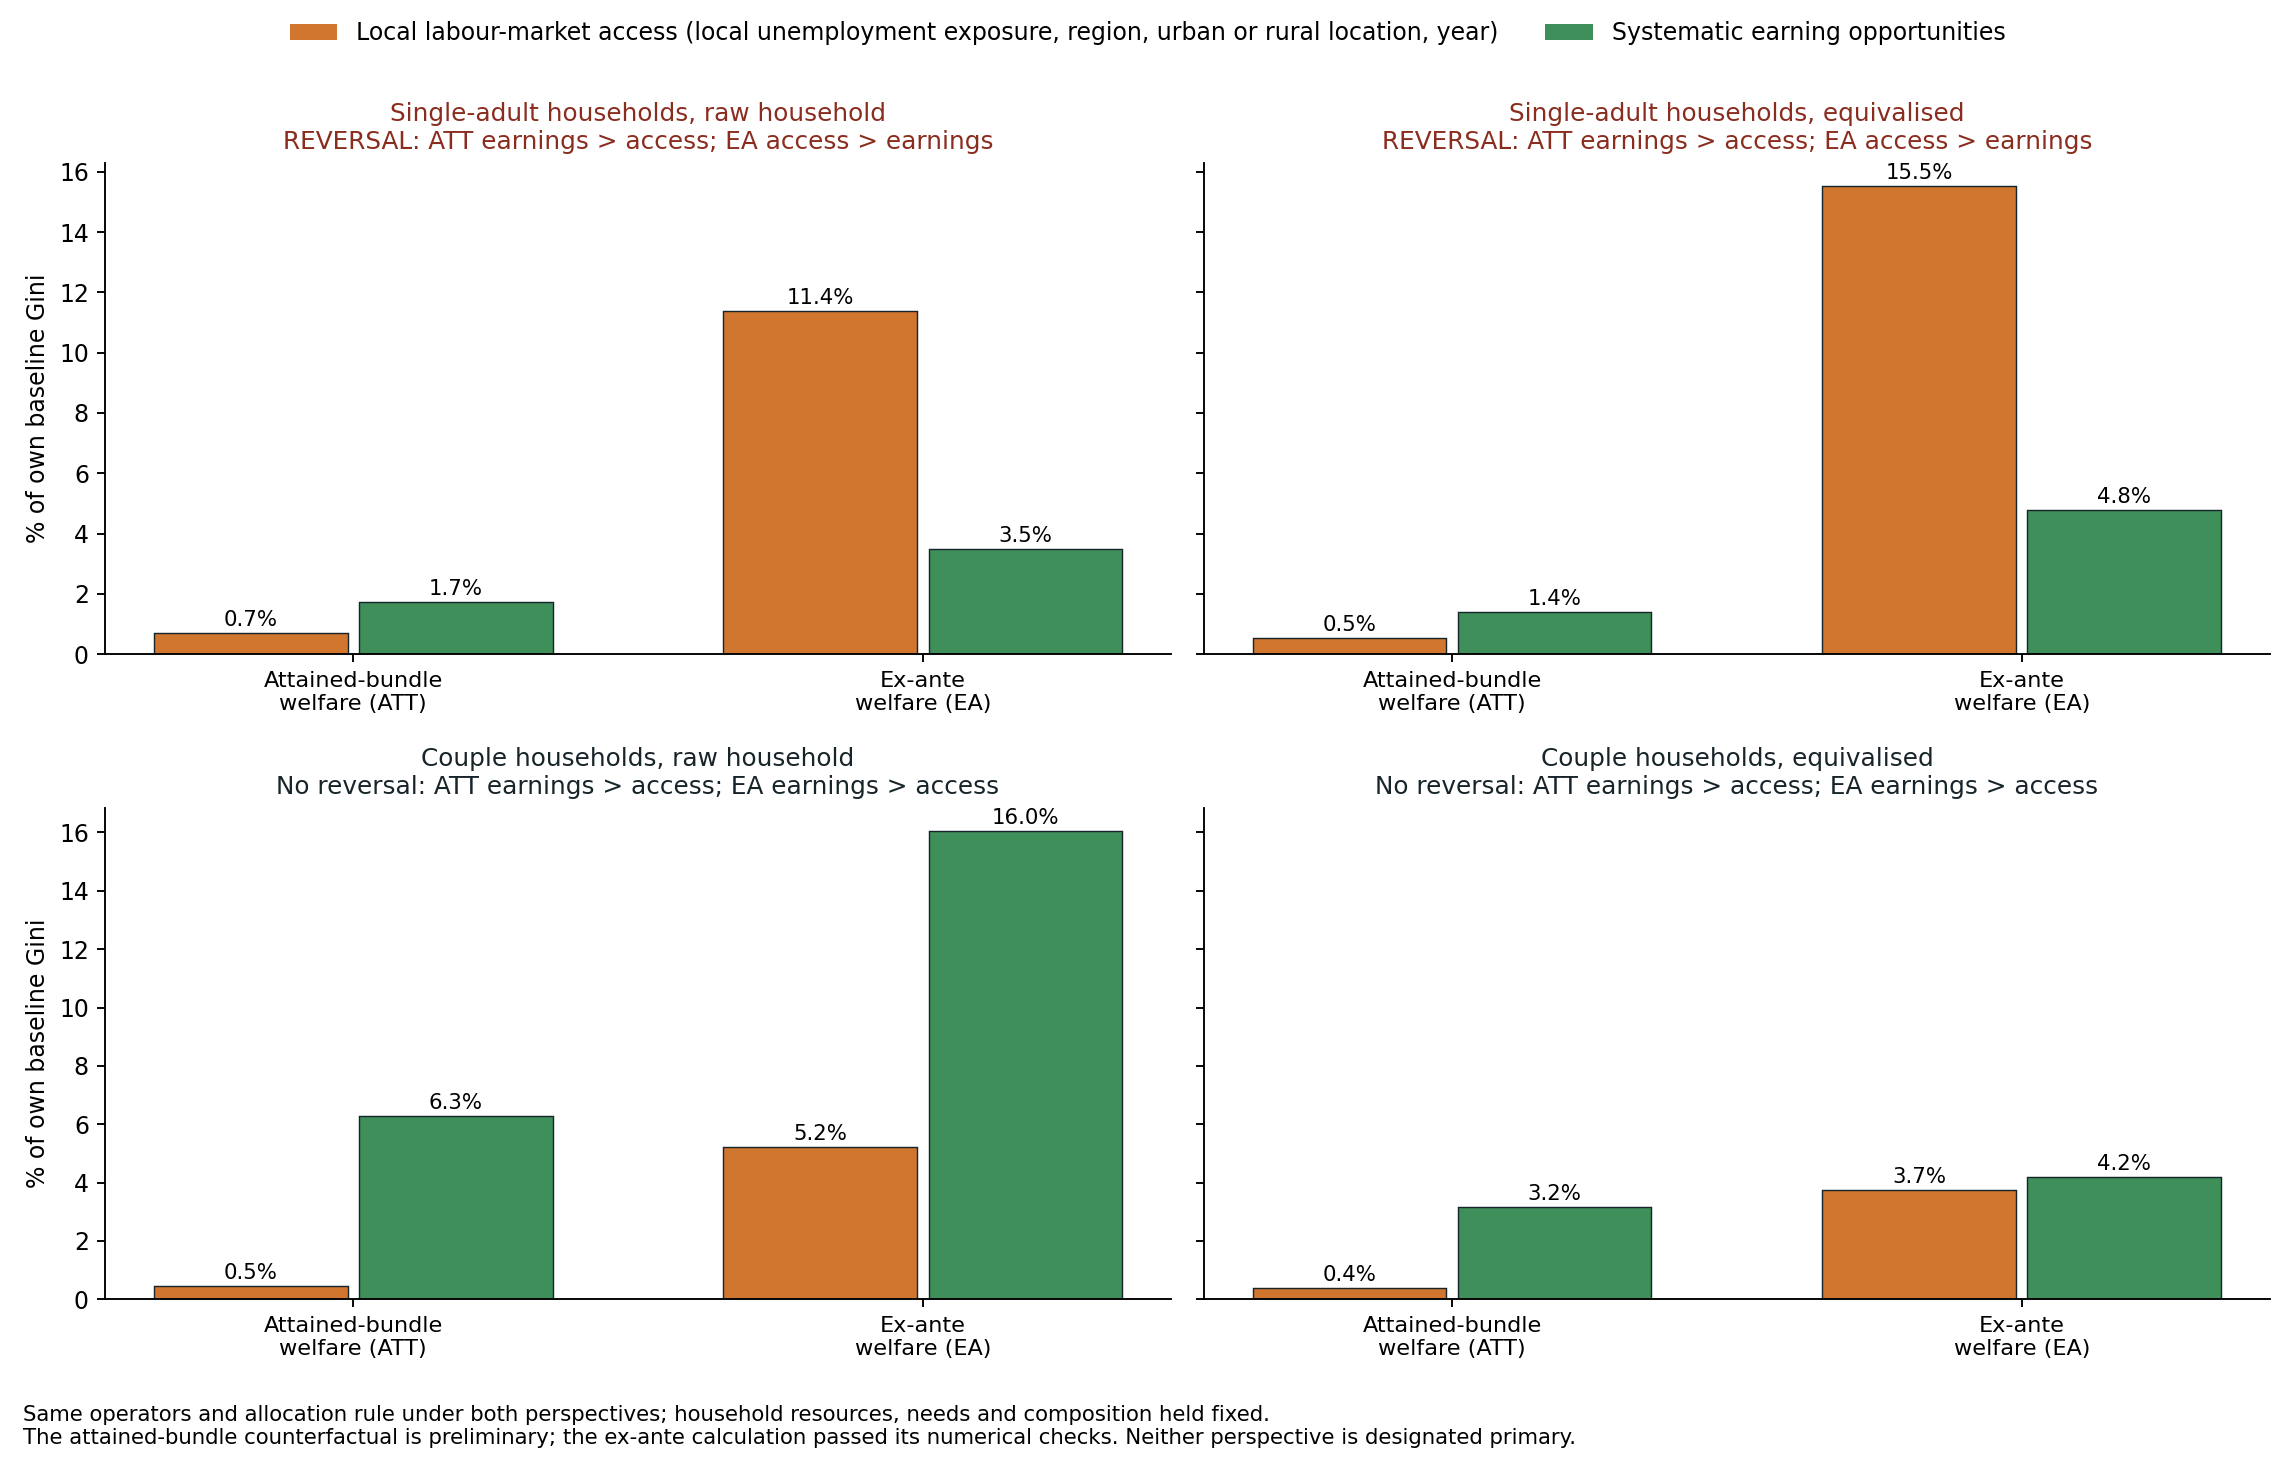
\includegraphics[height=0.57\textheight,width=\textwidth,keepaspectratio]{fig_v13_central_result.png}
\end{center}
\begin{columns}[T,onlytextwidth]
\column{0.46\textwidth}\centering
\textbf{\textcolor{chacc}{EA}: prospects}\\
{\footnotesize access + earnings \VEAOppMin{}--\VEAOppMax{}\% of baseline Gini}\\
{\footnotesize single adults: access $>$ earnings; couples: no reversal}
\column{0.46\textwidth}\centering
\textbf{\textcolor{chearn}{ATT}: attained outcomes}\\
{\footnotesize access + earnings \VAttOppMin{}--\VAttOppMax{}\% of baseline Gini}\\
{\footnotesize earnings $>$ access, both household types}
\end{columns}
\note{This is the result. Each panel shows the same two operators, local access
and earning opportunities, as a percentage of each perspective's own baseline
Gini, evaluated under the two welfare questions.

For single adults, access is the larger channel when welfare values the
prospect, about three times earning opportunities on both reporting scales, and
earning opportunities are the larger channel when welfare values the attained
outcome. For couples, earning opportunities stay in front under both: no
reversal.

The mechanism is the route by which opportunities enter. The attained-bundle
measure sees only the realised job, where the wage drives consumption, so
systematic differences in wage offers dominate. The ex-ante measure weights
every job by its availability, so the access environment enters welfare
directly. Why single adults reverse and couples do not is not tested here; one
reading is that a single adult's participation rests on one earner's access.

Prospects versus attained outcomes: two different welfare questions, and
neither perspective is designated primary. The comparison is also not a pure
contrast of definitions, because the two integrations use different designs.
The full tables are in the backup.}
\end{frame}

% ==================================================================== 15
\begin{frame}
\frametitle{What is not claimed}
\vfill
\begin{columns}[T,onlytextwidth]
\column{0.46\textwidth}
\centering
\textbf{Scope}\\[0.6em]
{\small Household resources, needs and composition held fixed}\\[0.5em]
{\small Access: local access, not total opportunity}\\[0.5em]
{\small Preliminary decomposition}
\column{0.46\textwidth}
\centering
\textbf{Not claimed}\\[0.6em]
{\small Not causal}\\[0.5em]
{\small No parameter uncertainty yet}\\[0.5em]
{\small Preferences are not responsibility}\\[0.5em]
{\small Neither perspective is designated primary}
\end{columns}
\vfill
\begin{center}
{\small prospects versus attained outcomes: two different welfare questions}
\end{center}
\vfill
\note{All the boundaries in one place.

The decomposition is preliminary: a restricted structural accounting exercise,
and the attained-bundle counterfactual integration is still being validated,
with short hours sparsely covered.

Nothing is causal. Separation rests on maintained functional-form and exclusion
restrictions, and no causal effect of geography, education or occupation is
estimated.

Parameter uncertainty has not been propagated through either decomposition, so
there are no confidence intervals on any share; repeat runs are simulation
checks.

The preference channel is not a responsibility channel. It contains a
reduced-form child term that can capture childcare constraints as well as tastes,
and deciding what people should be held responsible for is a normative step this
paper does not take.

Household resources, needs and composition are held fixed, and access is local
access, not total opportunity, so the shares are neither a complete
decomposition nor an estimate of everything unequal opportunity does.
Equivalisation is a convention and changes the couples results, which is why
both scales are reported. And the two welfare perspectives answer different
questions; choosing between them is a normative decision not made here.}
\end{frame}

% ==================================================================== 16
\begin{frame}
\frametitle{Conclusion}
\vfill
\begin{enumerate}\itemsep0.9em
  \item Choices reflect opportunities, not preferences alone.
  \item Prospects: access leads for single adults.\quad Attained outcomes: earnings lead.\quad Couples: no reversal.
  \item Restricted P/A/B: a bounded part of well-being inequality; preference sign not robust.
\end{enumerate}
\vfill
\begin{center}
{\small next: resources and needs as a fourth channel \quad$\cdot$\quad parameter uncertainty \quad$\cdot$\quad validation}
\end{center}
\vfill
\note{To close, the three answers.

First, observed choices carry information about opportunities: a model that
gives everyone the same jobs fits worse on the same households.

Second, the importance assigned to different labour-market inequalities depends
on whether welfare evaluates the opportunity prospect or the realised outcome.
Access leads for single adults when we value the prospect; earning
opportunities lead when we value the attained bundle; couples do not reverse.

Third, within the restricted decomposition, with resources, needs and
composition held fixed, local access and earning opportunities are a bounded
part of well-being inequality, and the preference contribution is not
sign-robust to equivalisation.

Next steps: household resources, needs and composition as a fourth channel;
propagating parameter uncertainty; completing validation of the attained-bundle
integration. Neither perspective is designated primary. Thank you.}
\end{frame}

% ============================================================ BACKUP
\appendix

% ==================================================================== B1
\begin{frame}
\frametitle{Backup: ex-ante decomposition}
\vfill
\begin{center}\small
\begin{tabular}{llcccl}
\toprule
 & scale & \textcolor{chacc}{access} & \textcolor{chearn}{earnings} & access + earnings & ordering \\
 & & Gini points & Gini points & \% of baseline & \\
\midrule
Single adults & raw & \VEASingPhiARaw{} & \VEASingPhiBRaw{} & \VEASingOppRaw{} & access $>$ earnings \\
              & equivalised & \VEASingPhiAEq{} & \VEASingPhiBEq{} & \VEASingOppEq{} & access $>$ earnings \\
\midrule
Couples & raw & \VEACoupPhiARaw{} & \VEACoupPhiBRaw{} & \VEACoupOppRaw{} & earnings $>$ access \\
        & equivalised & \VEACoupPhiAEq{} & \VEACoupPhiBEq{} & \VEACoupOppEq{} & earnings $>$ access \\
\bottomrule
\end{tabular}
\end{center}
\vfill
\begin{center}
{\small single adults: access $=$ \VEASingRatioRaw{} $\times$ earnings (raw), \VEASingRatioEq{} $\times$ (equivalised)}
\end{center}
\vfill
\note{The ex-ante numbers behind the central figure. Access plus earnings range
from \VEAOppMin{} to \VEAOppMax{} per cent of baseline ex-ante inequality,
depending on household type and scale. The calculation passed its numerical
checks, including an independent implementation. These are restricted
accounting shares with resources, needs and composition held fixed.}
\end{frame}

% ==================================================================== B2
\begin{frame}
\frametitle{Backup: attained-bundle decomposition}
\vfill
\begin{center}\small
\begin{tabular}{llcccl}
\toprule
 & scale & \textcolor{chacc}{access} & \textcolor{chearn}{earnings} & access + earnings & ordering \\
 & & Gini points & Gini points & \% of baseline & \\
\midrule
Single adults & raw & \VAttSingPhiARaw{} & \VAttSingPhiBRaw{} & \VAttSingOppRaw{} & earnings $>$ access \\
              & equivalised & \VAttSingPhiAEq{} & \VAttSingPhiBEq{} & \VAttSingOppEq{} & earnings $>$ access \\
\midrule
Couples & raw & \VAttCoupPhiARaw{} & \VAttCoupPhiBRaw{} & \VAttCoupOppRaw{} & earnings $>$ access \\
        & equivalised & \VAttCoupPhiAEq{} & \VAttCoupPhiBEq{} & \VAttCoupOppEq{} & earnings $>$ access \\
\bottomrule
\end{tabular}
\end{center}
\vfill
\note{The attained-bundle benchmark. Earning opportunities are larger than local
access for both household types and on both scales. Every coalition Gini and
contribution reproduces closely under an independent simulation run, and the
allocation closes to numerical precision; those checks validate the calculation
for the stated game, not its maintained assumptions. The preference
contribution changes sign with equivalisation in both samples, so no
directional claim is made about it. The lower part of the hours range is
sparsely represented in the integration sample, which is why this exercise stays
explicitly preliminary.}
\end{frame}

% ==================================================================== B3
\begin{frame}
\frametitle{Backup: matched households}
\begin{center}
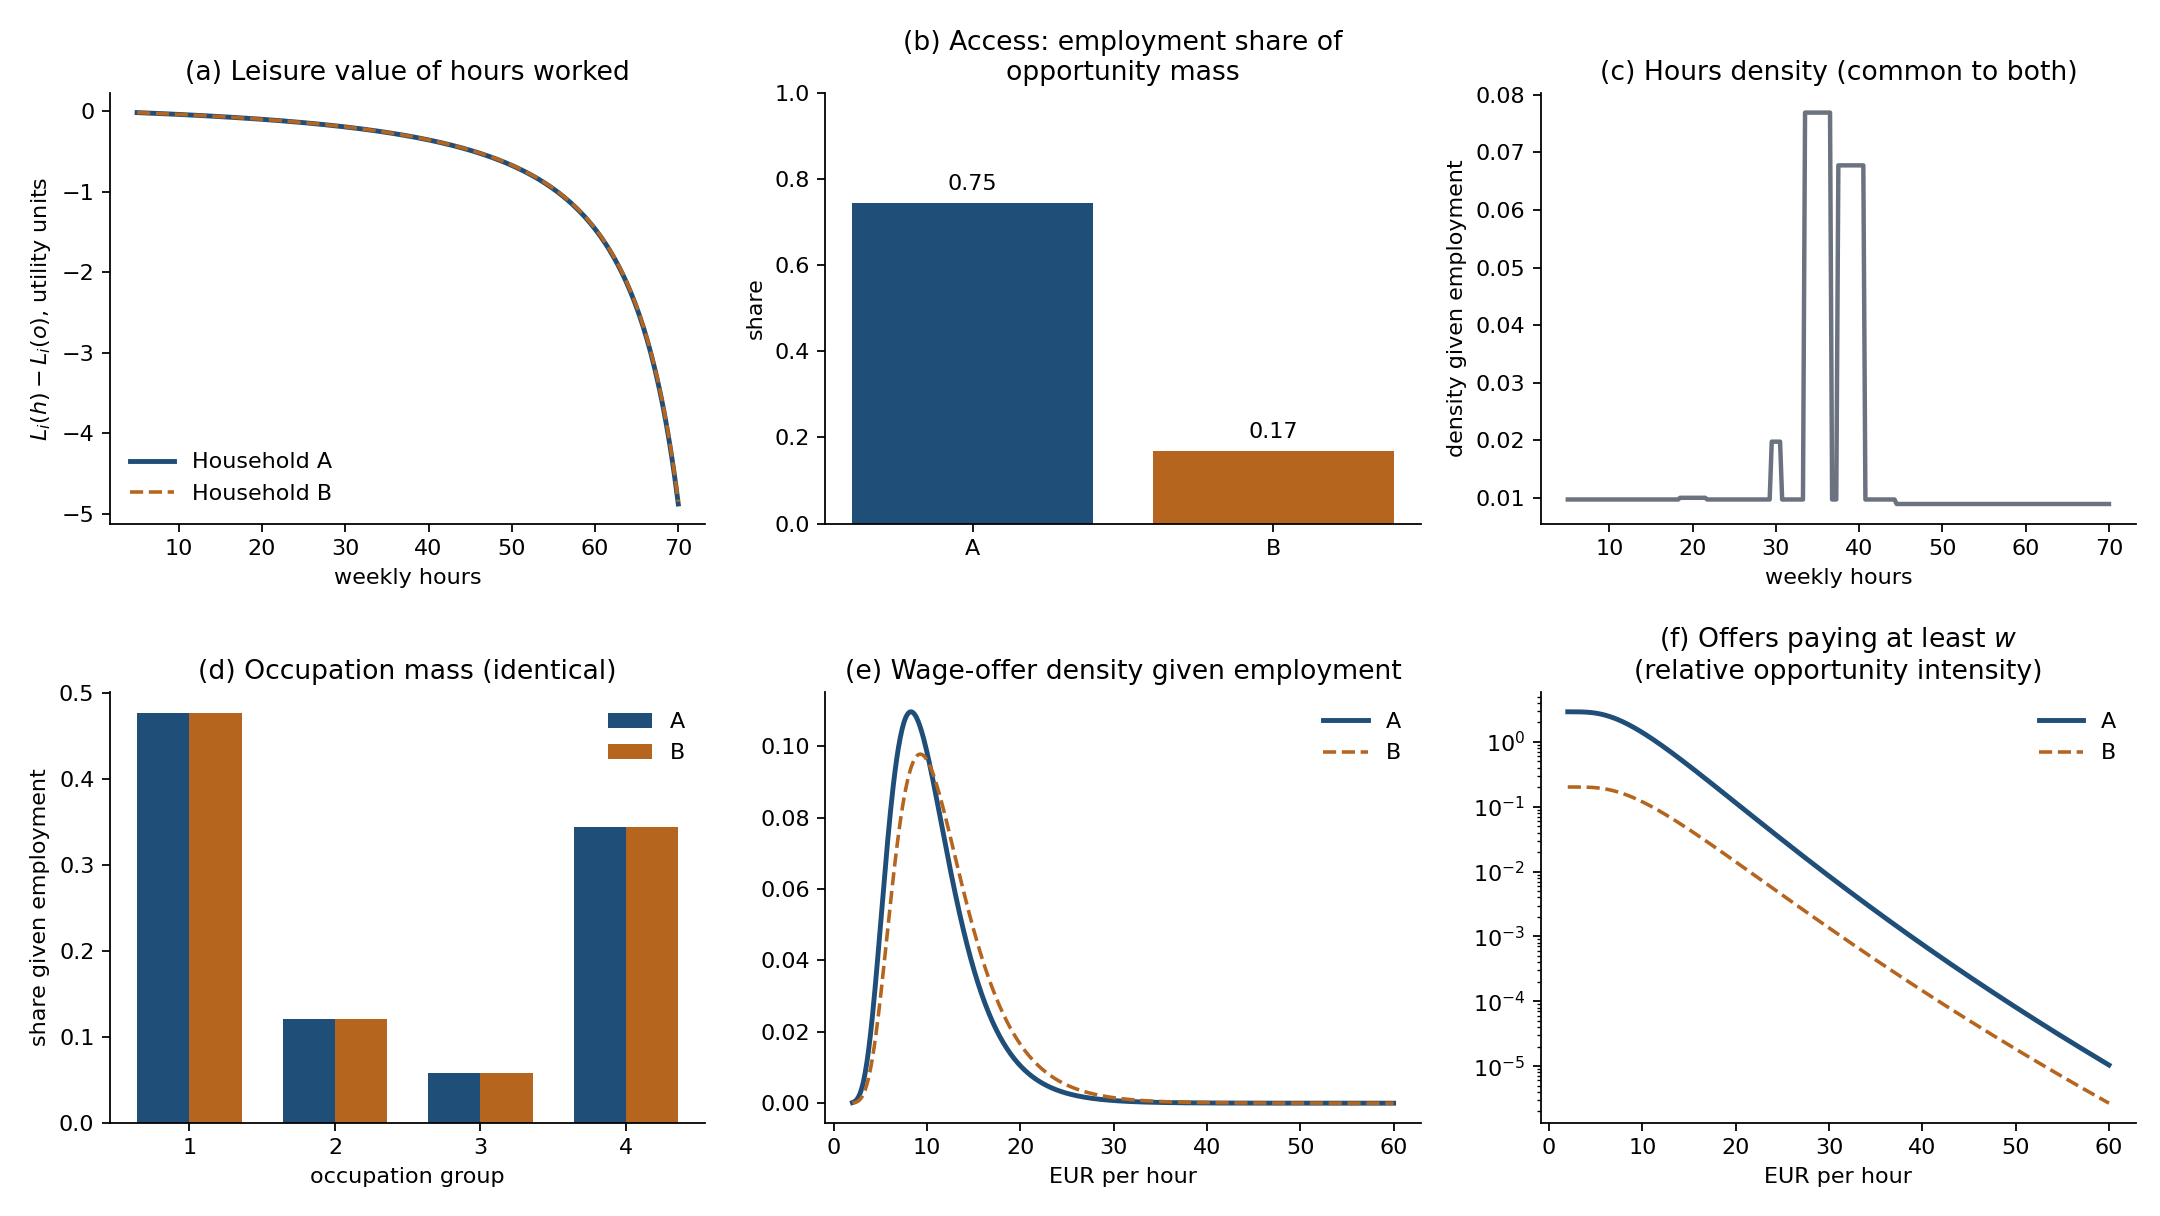
\includegraphics[height=0.66\textheight,width=\textwidth,keepaspectratio]{fig_matched_households_v11.png}
\end{center}
\begin{center}
{\footnotesize access: A $=$ \VMatchedAccessRatio{} $\times$ B \qquad wage-offer location: B $+$\VMatchedWageGap{} log points}
\end{center}
\note{What unequal opportunity means inside the model. Two employed single men
in the same occupation group, hours band and wage quintile, with nearly
identical estimated leisure profiles, selected by a stated rule: a teaching
example, not causal and not representative. If both were indifferent between
all jobs and not working, employment would be \VMatchedEmpShareA{} of A's
opportunity mass and \VMatchedEmpShareB{} of B's; the gap comes from local
unemployment exposure and region. B's wage offers are better, yet A faces more
offers paying at least any given wage over essentially all offer mass. Neither
is better placed on every margin; which one is better off depends on the welfare
question.}
\end{frame}

% ==================================================================== B4
\begin{frame}
\frametitle{Backup: equivalisation}
\vfill
\begin{columns}[T,onlytextwidth]
\column{0.46\textwidth}
\centering
\textbf{Couples, ex ante: access + earnings}\\[0.5em]
{\large \VEACoupOppRaw{}\% \quad$\longrightarrow$\quad \VEACoupOppEq{}\%}\\[0.3em]
{\footnotesize raw \quad$\to$\quad equivalised}
\column{0.46\textwidth}
\centering
\textbf{Couples, ex ante: preferences}\\[0.5em]
{\large \VEACoupPrefRaw{} \quad$\longrightarrow$\quad \VEACoupPrefEq{}}\\[0.3em]
{\footnotesize Gini points, raw \quad$\to$\quad equivalised}
\end{columns}
\vfill
\begin{center}
{\small modified-OECD scale: a convention, reported both ways}
\end{center}
\vfill
\note{Equivalisation is a normative convention and it is materially
consequential for couples under the ex-ante perspective: it moves the
access-plus-earnings share and turns the preference contribution negative. A
negative Shapley term means that, averaged over orders, equalising preferences
raises inequality; it does not show that preference heterogeneity is
equalising in any causal or welfare sense. That is why both scales are always
reported and no directional claim about preferences is made.}
\end{frame}

\end{document}
